Throughout all of the various aggregation methods covered with and without experimentation, trying to find good ideas and sensible applications of them has been an end goal.
Ultimately, none of the robust aggregators have performed as well as I would have liked on the higher numbers of malicious clients and tend to have reduced accuracy if anything.
This lead me down the path of trying to use ideas from current aggregators and methods in federated learning to try to improve on the SotA.
\\ \\
My goals for creating a better robust aggregator are:
\begin{itemize}
    \item Better understand the robust aggregator space in federated learning.
    \item Enhance current aggregation methods through clustering.
    \item Handle more malicious clients than any other robust aggregator.
    \item Be able to handle free-riders better than other aggregators.
\end{itemize}
Throughout all that I wish to include in the aggregator, I name it FedPADRC (Personalised and Adaptive Dimension Reducing Clustering).


\section{Clustering}
Initially, I thought about clustering similar models together through K-Means Clustering.
Similar ideas like this have been tried already \cite{cluster_robagg} but didn't really attempt anything that I would personally call robust (even if they claimed otherwise).
So, I wanted to build upon this idea by instead using some combination of FedAvg, COMED and MKRUM to do the aggregation.
I couldn't really use AFA of FedMGDA++ as they both relied on learned information about the whole system.
FedMGDA++ especially relied on having all the clients present at every step on never subsets of the clients.
\\ \\ 
However, robustly aggregating at only the clustering stage seemed like it would very easily be abused by a coordinated attack of malicious clients.
This is because malicious clients would end up having similar models due to their coordinated attack strategy being the same.
Therefore, there would always be at least one cluster of just malicious clients.
Something like COMED might be able to handle this better but it was something definitely worth investigating.
So, I would then also need to have robust aggregation happen when aggregating the cluster centres together to form the end model (something that hadn't been done before).
\\ \\
Prior to any testing, one thing that is important to bring up is that K-Means Clustering is a very computationally intensive algorithm to run.
Increasing the number of clients beyond the 30 here to systems with orders of magnitudes of more clients might not be a sustainable process.

\subsection{Aggregator Capabilities}
There are 9 different combinations of aggregators that I can try but realistically having FedAvg be the aggregator in the second aggregation step is pretty futile as malicious clients are pretty guaranteed to get through and damage the model.
Also, for trying to segregate the clients' models from each other, more training than the standard 2 epochs will need to be done.
So, I increased the number of epochs per round to 10 when we're clustering so that each client's model can appropriately represent itself before it is clustered.
\\ \\
Very early on it appeared to be apparent that using MKRUM as an external and internal aggregator proved pretty much useless.
This was because with just 1 attack, it's performance was all over the place [\ref{fig:mkrum_bad}] with any internal aggregator.
However, COMED on the other hand seemed to steam-roll right through any number of malicious clients, only starting to fail at around 22 malicious clients.
This is incredible as this outperforms any of the other robust aggregation methods tested!
\begin{figure}[htbp]
	\centering
    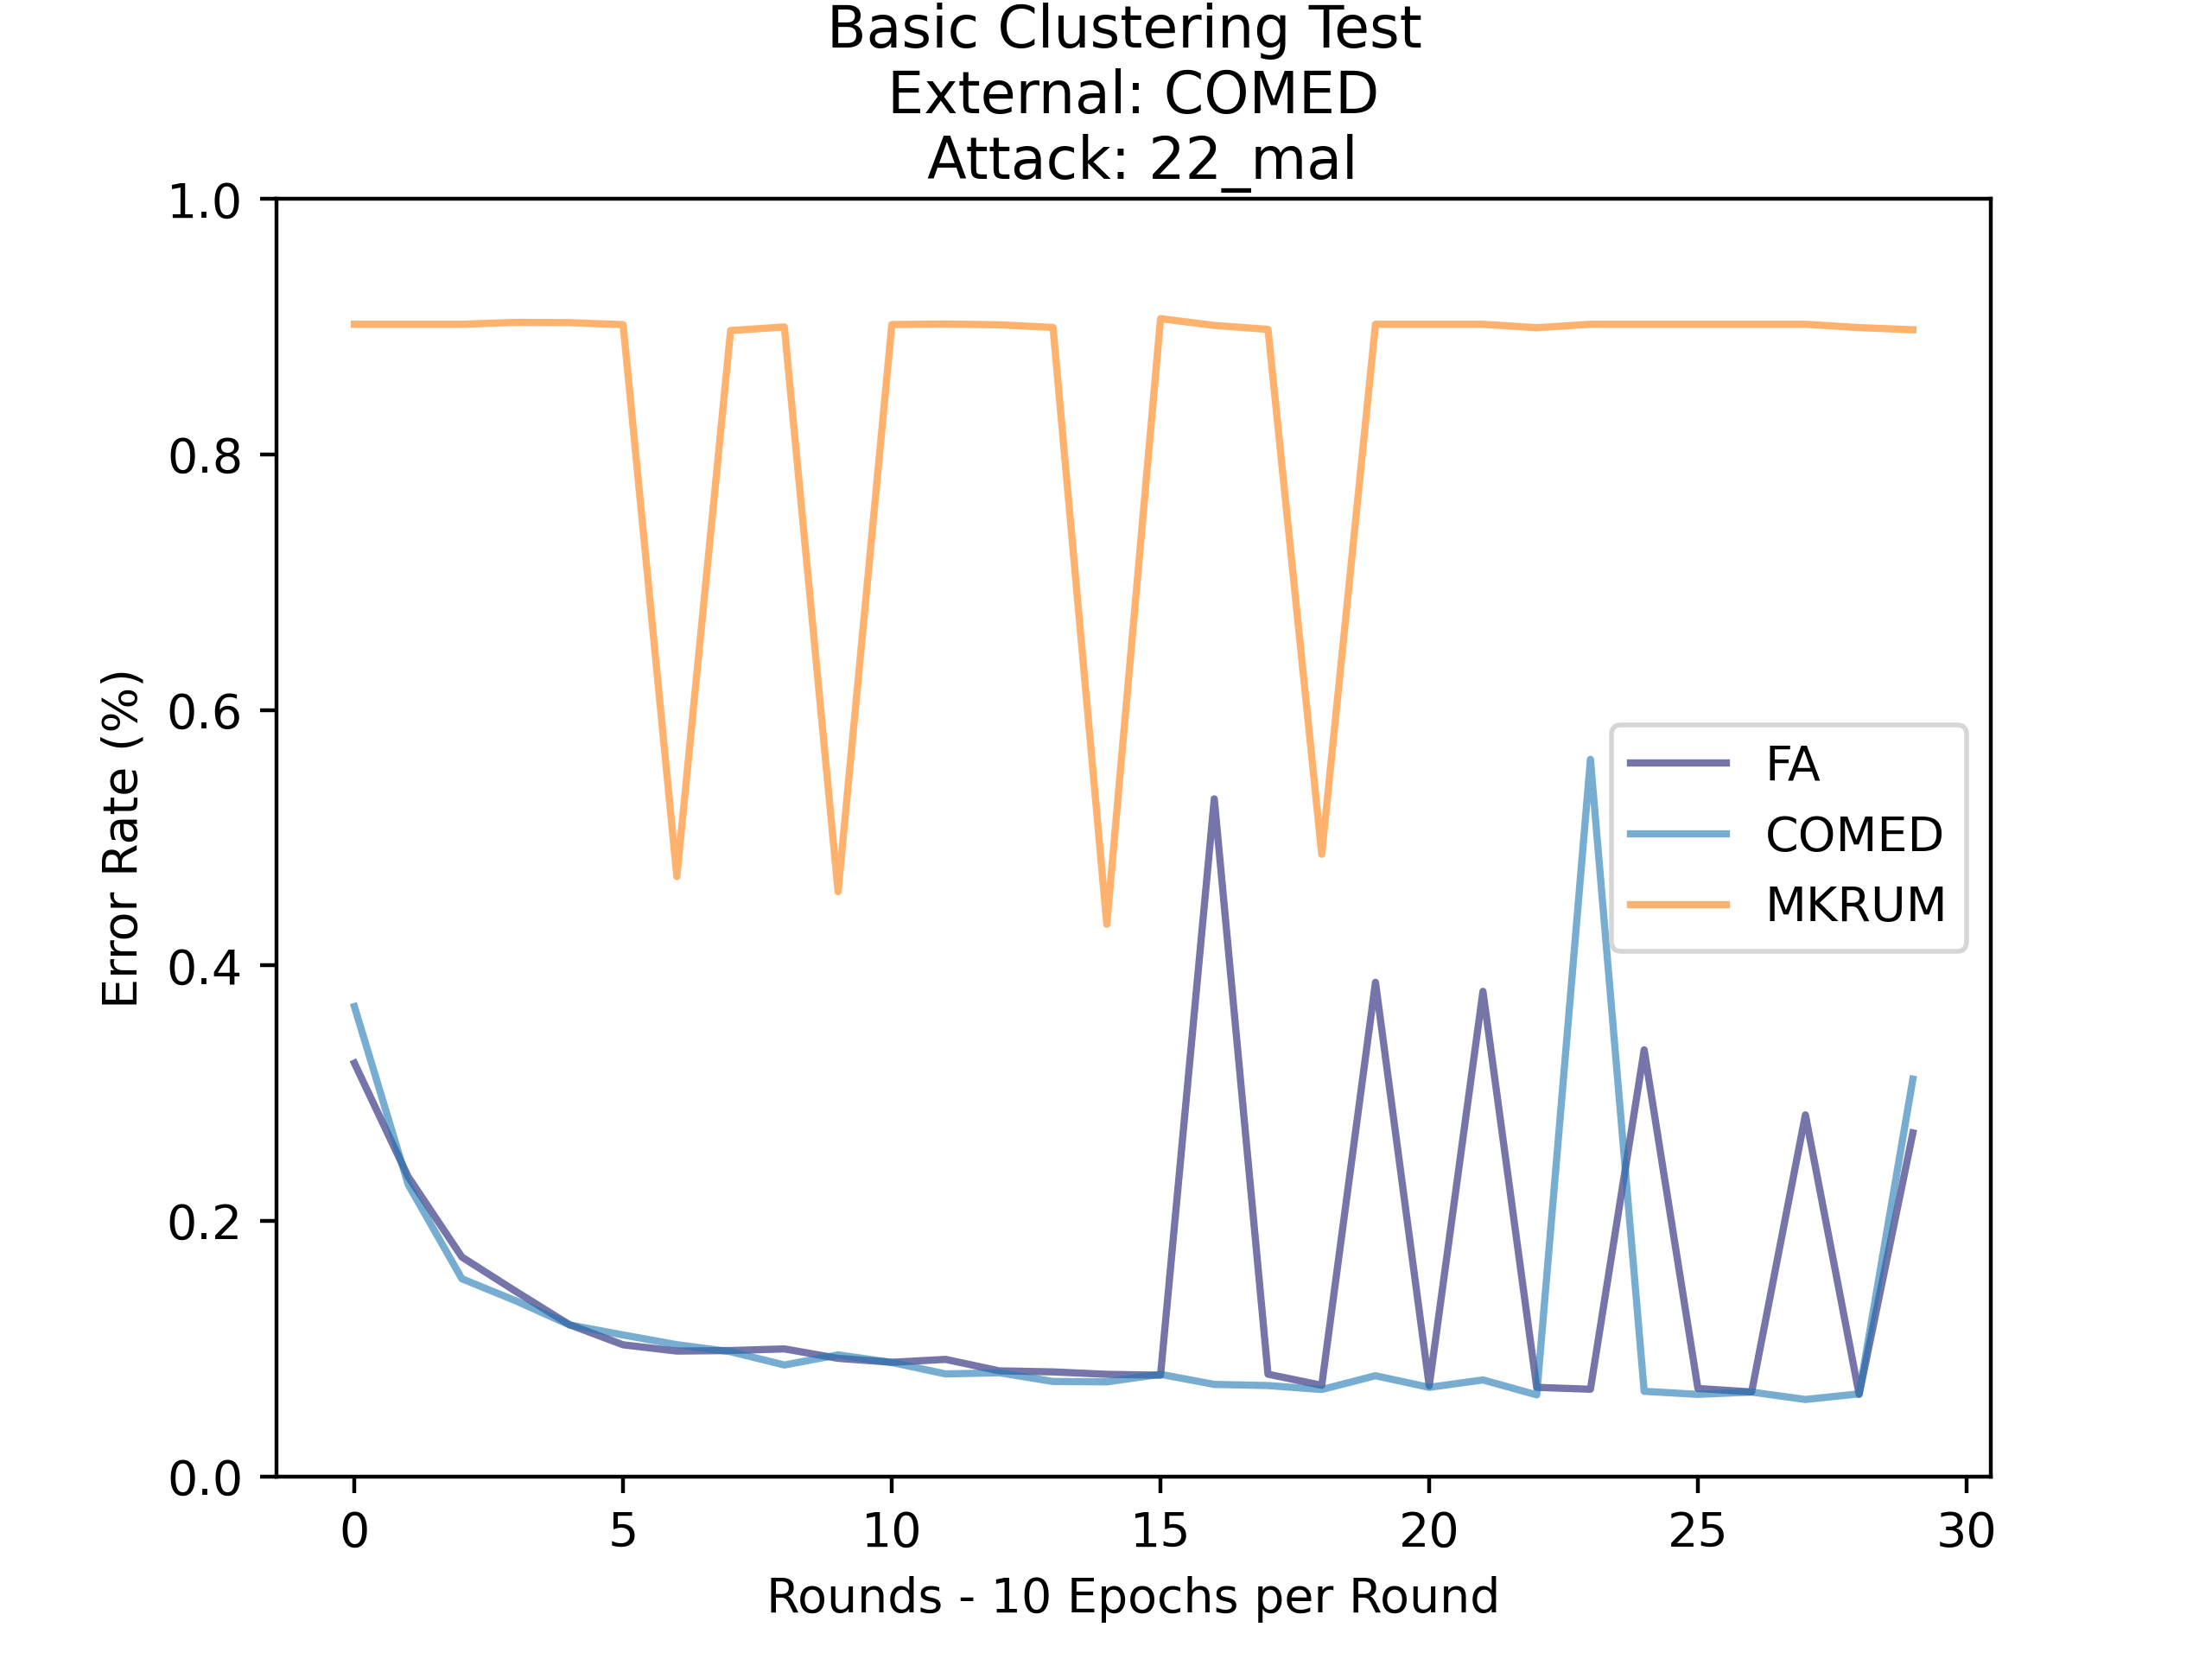
\includegraphics[scale=0.5]{my_agg/graphs/cluster_comed_22.png}
	\caption{Error Rate of K-Means Clustering with COMED as the External Aggregator - 22 Malicious Clients}
	\label{fig:comed_22}
\end{figure}
Throughout testing, both FedAvg and COMED performed similarly in their internal ability to aggregate, with it only varying later on.
One thing to note is that when the data is non-IID, it might not be as simple as that and FedAvg might start to outperform COMED through its increased data use.
\\ \\
What's also interesting to see is the extremely quick convergence of the model.
This is most likely due to no interference from the malicious clients in the first half of the total number of rounds.
You can also clearly see that the model itself is over-fitting and should realistically only be lasting for 10-15 rounds or so.
This would then help with the later stage spikes that we see.
\\ \\
It didn't quite end there though, as for some very strange reason, MKRUM's performance appeared to get better with more malicious clients being added.
This was such that I was seeing performance from MKRUM being used as an external aggregator compared to COMED at more than 22 malicious clients.
Now, this doesn't then lead me to believe that overall MKRUM performs better, just that it has its very unique and weird moments of performance.
Overall, I believe that using FedAvg to aggregate the clients within the clusters and using COMED to aggregate the cluster centres is the best way forward.


\subsection{Finding the Optimal K}
When it comes to K-Means Clustering, finding the best K-value to use is extremely important to ensure that the data is properly split up and segmented.
Luckily, it is not a particularly complex task and normally just requires testing out the different K-values and using something called the "Elbow Method" to determine which is the best.
\\ \\
The elbow method is when you plot the the number of clusters against some distance/scoring metric.
This could be their literal distance, sum of squared distances, based on accuracy etc.
In plotting there will be a more highlighted point [\ref{fig:elbow}] where the rate of change drastically decreases.
This indicates that further increases in the K-value result in not much benefit and would most likely be over-fitting the data.
\begin{figure}[htbp]
	\centering
    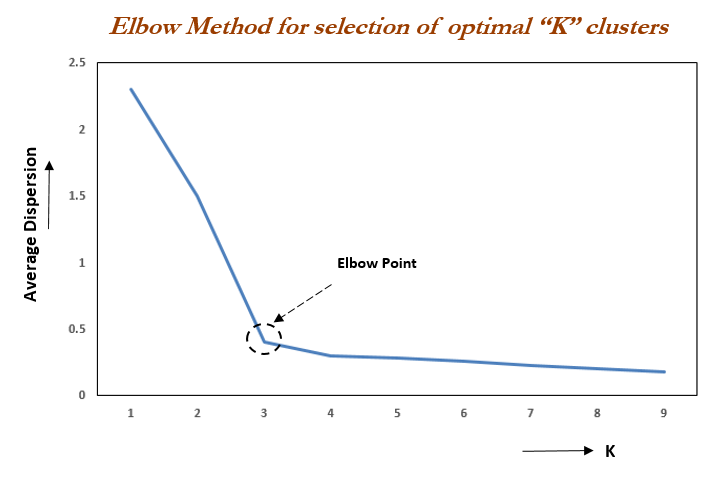
\includegraphics[scale=0.5]{my_agg/graphs/elbow.png}
	\caption{Elbow Method with Highlighted Optimal K-value \cite{oreily_elbow}}
	\label{fig:elbow}
\end{figure}
\\ \\
For the scoring metric I decided to plot the sum of the distances that each model is away from its designated cluster and total it for each value of K from 1 to 30.
Now, there are definitely less hard-coded solutions than this and ultimately using a solution that would have this K-value change would be the most ideal.
However, to recalculate this at every federated round takes minutes for even small models like with MNIST.
So, realistically trying to get a rough idea of the values of K that would be more desirable is the more sensible choice.
\\ \\
Funnily enough, there ended up not being any particular point that could be realistically identified as the elbow point.
I did the above calculations for no attacks, 5 and 20 malicious at rounds 0, 5 and 20 [\ref{fig:k_elbow}].
This was so that I was able to see how representation of the data changed throughout so I wasn't simply basing my analysis from 1 point.
\\ \\
Under no attacks, the line was a constant gradient on average and gave no hint of an optimum point.
Under 5 malicious there were similar characteristics but with a slightly steeper descent at first, potentially hinting at some K-value around 4.
At 20 malicious is where things get weird and it is almost like a K of 2 is the best.
\\ \\
Interpreting these results is interesting to say the least, but one last method I can try is to see what the final and/or minimum error rate values are at each K and see if that can shed any more light on the situation.
What I am expecting is that there won't be much difference with 0 attacks but having a good K value will be more and more important with 5 and 20 as that is where you'll see damage starting to be being done.
\begin{center}
    \begin{longtable}{ |c|c|c|c|c|c|c|c|c|c|c|c|c| }
    \caption{Error Rate (\%) as K Changes}
    \label{tbl:k_error_rate}
    \hline
    K & 1 & 2 & 3 & 4 & 5 & 6 & 7 & 8 & ... & 15 & ... & 30 \\ \hline
    \multicolumn{13}{|c|}{} \\ \hline
    0-Min & 5.3 & 7.4 & 5.7	& 5.7	& 5.4	& 5.3	& 5.3	& 5.1 & ...	& 5.4 & ... & 5.4 \\ \hline
    0-Final & 5.3	& 7.9	& 5.8	& 5.8	& 5.4	& 5.5	& 5.6	& 5.1 & ...	& 5.4 & ...  & 5.4 \\ \hline
    \multicolumn{13}{|c|}{} \\ \hline
    5-Min & 8.8 &	90.2 &	14.1 &	9.4 &	7.2 &	6.5 &	6.3 &	6.0 & ... &	5.6 & ...  & 7.3 \\ \hline
    5-Final & 28.6	& 90.2	& 16.2	& 9.4	& 7.9	& 6.5	& 6.3	& 6.0 & ...	& 5.8 & ...  & 7.5 \\ \hline
    \multicolumn{13}{|c|}{} \\ \hline
    20-Min & 90.2	& 90.2	& 13.4	& 9.4	& 7.3	& 7.4	& 6.5	& 6.4 & ...	& 25.4 & ...  & 89.7 \\ \hline
    20-Final & 90.2	& 90.2	& 16.39	& 9.82	& 8.24	& 7.4	& 6.72	& 11.9	& ...	& 26.94 & ...  & 90.2 \\ \hline
    \end{longtable}
\end{center}
Through setting the number of rounds to 15 to stop over-fitting and remove the peaks near the end, we can now see how the solutions perform at various points in Table \ref{tbl:k_error_rate}.
Seeing the no attack error rates really seemed to fit perfectly with the previous test done as the value doesn't change too much [\ref{fig:k_elbow_0}] except when K is 2.
After about the halfway point, K seems to do a little worse as well on average, indicating that it's probably become too high (although it's very minimal).
\\ \\
Where things start to change a bit is when we increase the number of malicious clients to 5.
Here, we now notice [\ref{fig:k_elbow_5}] that K has to be a minimum of 3 for the clustering to work properly.
Going any higher than 6/7 gives no improvement and would be overkill in this situation.
It should be noted that right at the very end, when the algorithm is essentially just COMED by itself, there is a gentle increase in the error rate.
\\ \\
Finally, we hit some good data with 20 malicious clients [\ref{fig:k_elbow_20}] as there is a proper U-shape to the error rate.
This further highlights that between 3 and 5 is the optimum number for K with the elbow-point being at about 3 or 4.
Noticing that the final value at K=3 is slightly higher than the minimum value suggests that the solution there is getting a bit worse nearer to the end of the federated rounds.
This leads me to conclude that a K of around 5 is the optimal for this instance but in general terms, values between 3 and 7 should probably work fine.




\section{Dimension Reduction}
When it comes to clustering the data, performing it on the entire model's parameters is very much a noisy affair as there will be plenty of parameters that aren't very important.
What we then end up with, is a clustering that relies on a bunch of noise to be performed.
For a point of reference, the MNIST model that I am using contains 535818 different parameters (with larger models getting into the millions).
Realistically, there are only going to be a certain number of parameters that are actually useful and will contribute to the clustering properly.
\\ \\
Current methods through using a VAE exist but only alongside SAD and they don't fully utilise the pure lower-dimensional form that is created and is instead used for reconstruction.
Not only this, but the hyper-parameter fine-tuning that must go into such a model (e.g. number of layers, layer size etc.) provides a more variable solution that must be curated.
They also require training to be accurate and so aren't going to be as effective early on in the aggregation.
\\ \\
However, that doesn't mean they aren't useful.
VAEs are great when you do want to reconstruct data (and maybe compare that way) but ultimately that is not the goal that I am trying to achieve here.
This is where Principal Component Analysis (PCA) comes in.
PCA is a quick and effective form of dimensionality reduction that can create a more concise representation of our models.

\subsection{Number of Dimensions}
The only parameter that can really be chosen for PCA is what dimension should the data be represented in.
We could perform similar tests that were done for K-Means but luckily PCA provides a handy little thing called "Explained Variance".
This is essentially just sum of squared distances but in more mathematical terms it is used to measure discrepancies between the representation via PCA and the actual data.
This works very nicely for us as we want to keep as much useful information as possible without over-fitting.
\begin{figure}[htbp]
	\centering
    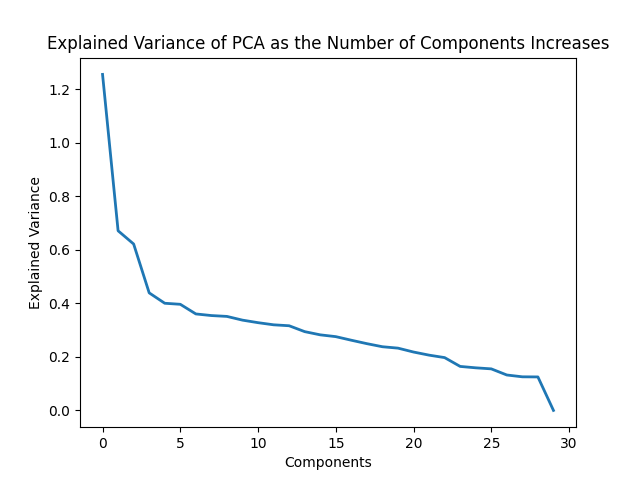
\includegraphics[scale=0.5]{my_agg/graphs/0_r0.png}
	\caption{Explained Variance with No Attacks at Round 0}
	\label{fig:pca_00}
\end{figure}
\\ \\
As seen in [\ref{fig:pca_00}], we can start to see that a dimension value of around 1-4 is probably the sweet spot.
Other rounds later on [\ref{fig:pca_01}, \ref{fig:pca_02}] may appear to indicate that actually we don't want to perform PCA at all.
However, this pattern only really appears when there are no attacks present and as soon as we start adding some, it becomes more apparent [\ref{fig:pca_50}] that this is not the case.
Instead, we end up seeing that a dimension value of 1 looks to be a pretty safe bet with some potential at round 2-4.


\subsection{Low Dimensional Beings}
As has become apparent, relying on traditional methods to guarantee what the optimal values are, is not always the best idea.
So, to help further guarantee that the low PCA dimension values are correct, let's plot the coordinates of the PCA transforms of these values and see how they compare.
We can only do this in 1D, 2D, 3D and 4D but seeing as it theoretically shouldn't need to go beyond this anyway, it should be fine.
It should be noted that the 4th dimensions is represented by size of the plotted points in the graphs.
\\ \\
With no attacks you get pretty much what you would expect [\ref{fig:0mal_dims}] and all 4 dimensions show to add some level of useful information.
When we start adding attacks, we would expect that the most information gain happens from 1D and that is pretty much what you get at an initial glance.
\begin{figure}[htbp]
	\centering
    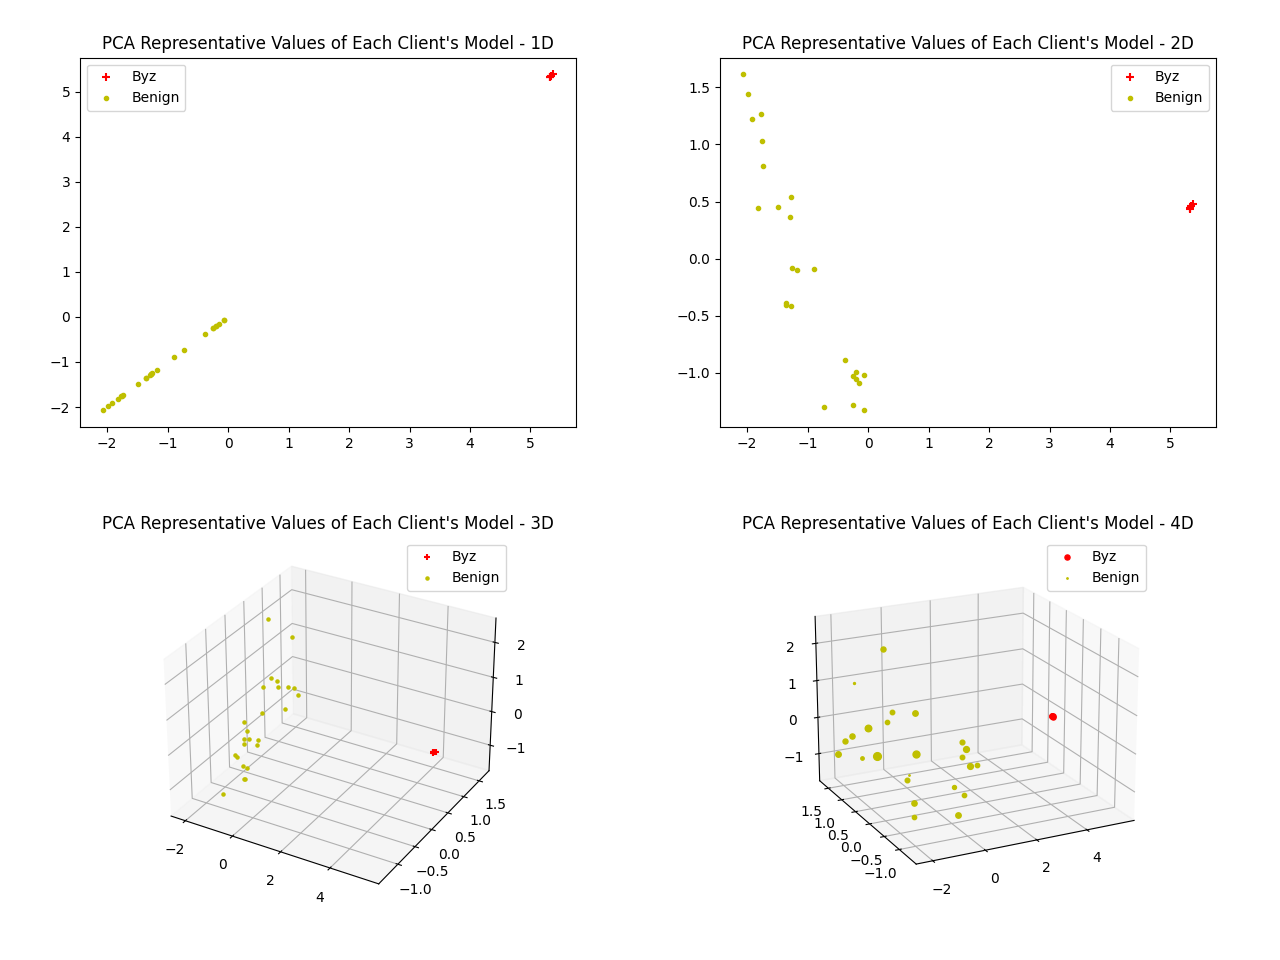
\includegraphics[scale=0.33]{my_agg/graphs/5mal_dims.png}
	\caption{PCA Transform Positions over Four Dimensions - 5 Malicious}
	\label{fig:5mal_dims}
\end{figure}
As shown in Figures \ref{fig:5mal_dims}, \ref{fig:20mal_dims}, we see that the remaining 3 dimensions all have the malicious clients placed in the middle of the same region [\ref{fig:4d_diff}] in their respective dimensions.
However, what becomes important is the scattering of the benign clients.
In all other dimensions they are far more unique, which lends them to not be clustered with the malicious clients even if the first dimension were to fail at separating the 2 groups.
This is also seen in practice, where the accuracy of 1D solutions tends to end up including more malicious clients as time goes on, showing that the segmentation isn't working as well as the Explained Variance would have you believe.
\\ \\
This is most likely due to the global aggregation sharing the global model out to every client, softening the malicious clients and making them appear more benign in the process.
This causes their PCA transform values to spread out more, increasing the likelihood that more clusters will be assigned to them.
This \textit{can} be mitigated through increasing the number of epochs per round (that's why 10 is used instead of 2) but it isn't a perfect solution.
We are currently able to fix this through using 4 dimensions for the PCA but there is obviously something about 1D PCA that seems so tempting.
\\ \\
Increasing the number of dimensions doesn't really fix this and at higher dimensions (e.g. 10 [\ref{fig:dim10_26mal}] or 29 [\ref{fig:dim29_26mal}]) we still some spiking at later federated rounds.
The error rate is also not as smooth and is more susceptible to be jagged throughout, indicating that the current algorithm isn't as robust.



\section{Personalisation}
We nicely fall in the lap of federated learning personalisation.
We have hypothesised that the 1D PCA option might not be working as well simply because the malicious clients are getting good updates that makes them appear more benign over the course of the federated rounds.
This can be seen in Figure \ref{fig:mal_spread} as the spread is more segmented in 2D while in 4D there is only 1 dimension of spread that is much less segmented
So ideally, we don't want to give any malicious client a global update that will inevitably work against the benign clients.
\begin{figure}[htbp]
	\centering
    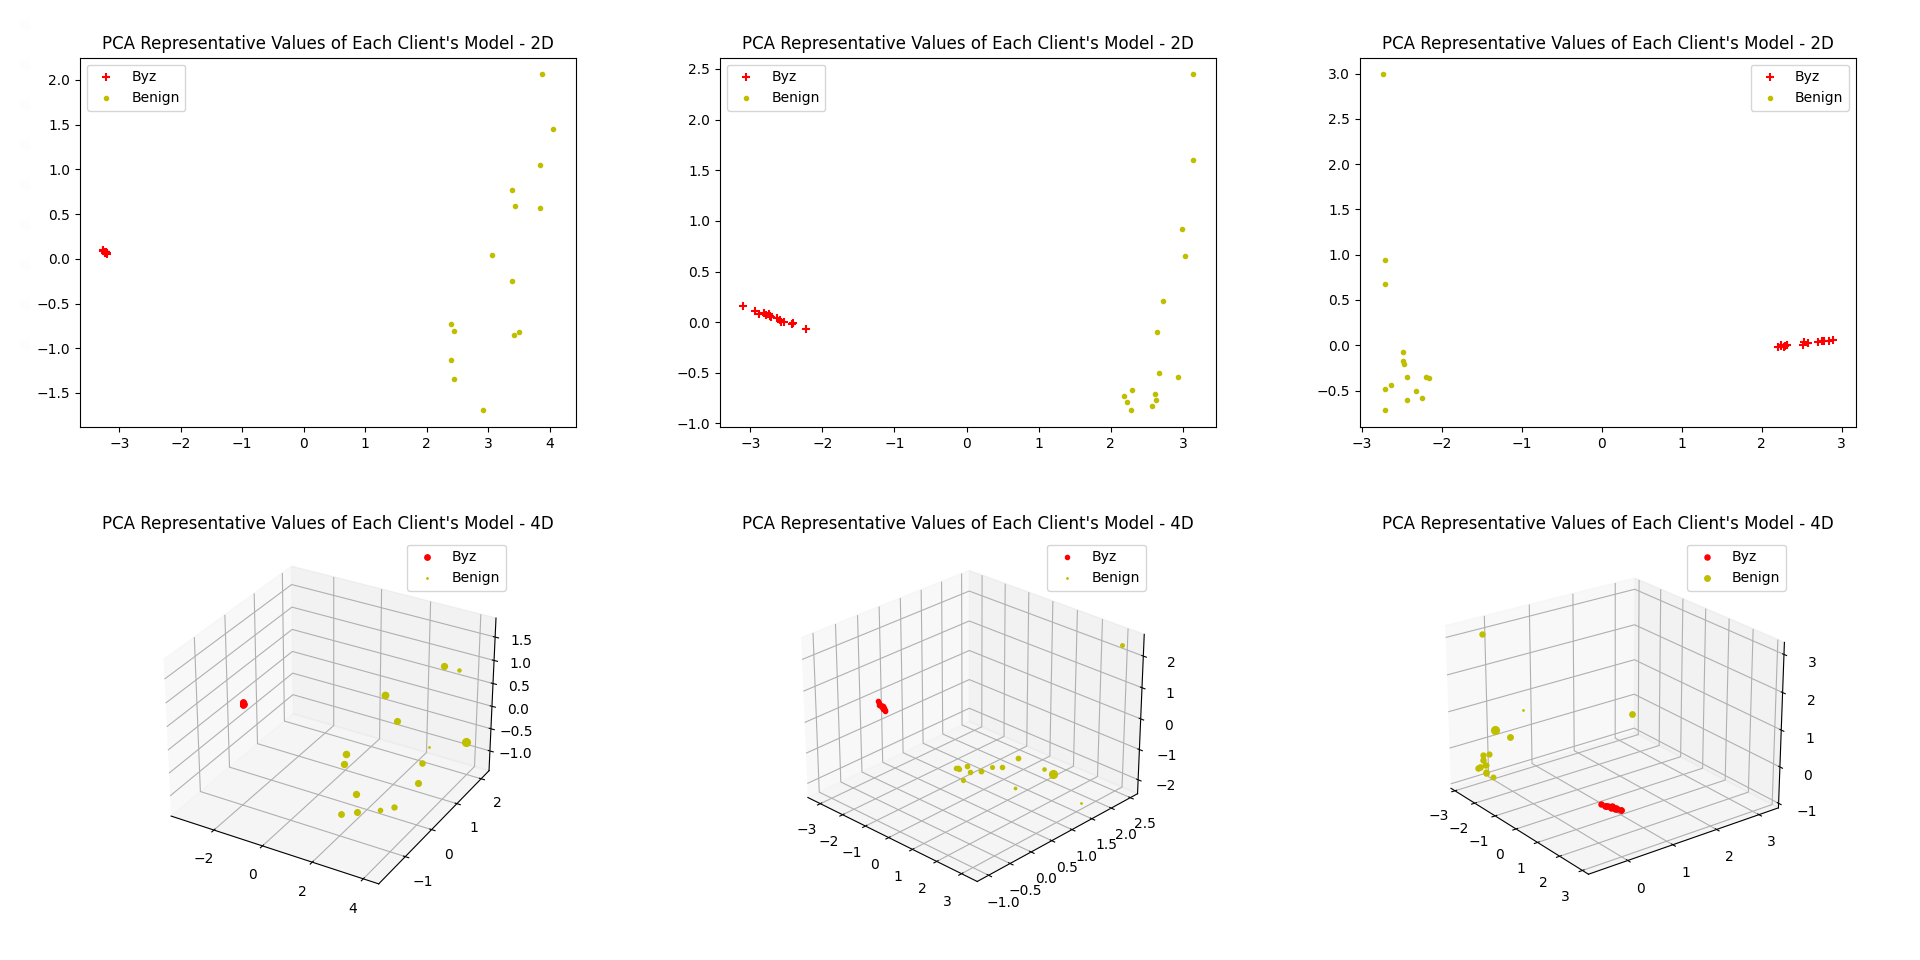
\includegraphics[scale=0.2]{my_agg/graphs/mal_spread.png}
	\caption{PCA Transform Position Spread for 2D (top) \& 4D (bottom) in Rounds 0, 1, 2}
	\label{fig:mal_spread}
\end{figure}
\\ \\
This is where the idea of personalisation comes in.
We either don't want to update certain clients or simply update them with less useful information that is specific to them.
This also gives us the capability to not have to use COMED to do the robust aggregation as we would already be robustly aggregating in the first place.
However, it may end up being more beneficial to also use COMED on top of this.



\subsection{Methods of Personalisation}
There are 4 main ways that I have come up with to achieve this, with the names that I will be using to refer to them as in the brackets:
\begin{enumerate}
    \item Selective Update (selective): this method involves only updating a select number of the clients at each round. This number would be determined by the floor of half of the number of clusters + 1. E.g. 3 for 5 clusters, 4 for 7, 5 for 9, etc. (we will assume 3 for K=5 from here on out).
    This would then hopefully lead to the malicious cluster not being updated (along with a benign one potentially) and the other clients in the selected clusters get an aggregated model of the top 3 clusters.
    \\ \\
    This would end up causing the main 3 clusters to get updated with data from each other, ultimately having them remain more similar and therefore more likely to update again together in later rounds.
    This would then help reduce the benign poisoning that is given to the malicious clients to help them.
    
    \item Concentrated and General Updates (general): here, we do 2 different global model updates.
    One is concentrated model of the top 3 best clients (as described above) and the other is a more general model from the aggregation of all of the clusters.
    Instead of just sending the concentrated model out to the best clients, it then gives the left-out benign cluster an opportunity to contribute to the other benign clusters later on, while still hopefully keeping the top 3 best clusters away from the malicious cluster.
    \\ \\
    This might not work as well, as the malicious client is still getting updated.
    There is also the possibility of then causing the best clusters to become too similar such that they merge and give a higher likelihood for the malicious clients to form more than one cluster.
    It will almost definitely cause the non-best benign cluster to then get polluted with damage from the malicious cluster as it will have received the general update which will include the malicious cluster in the aggregation.
    
    \item Thresholding (thresholding): instead of just using the best 3 out of 5, instead we figure out which clusters are more than a set number of StDs away from the mean and then set their weighting to 0.
    This allows us to then aggregate on the rest of the data with their own personal weighting so that in theory, you get to fully aggregate on all of the benign clients' data, instead of just some of it.
    \\ \\
    This could also be applied in conjunction with the previous method such that the general model could then be aggregated on all non-0 weighting clusters while the concentrated model is still formed.
    You then also have the option to not update the 0-weight cluster at all like in the first method.
    
    \item No Global Model (no global): if we were to just not aggregate the clusters' models together, then in theory each client would get a more personalised model that was best suited to them.
    It would also keep all of the malicious clients building their own malicious model while all of the benign clients build their own separate ones.
    This would help minimise any form of cross-over between the clusters but it wouldn't allow for as much model generalisation.
    Depending on each client's end goal, this might not be an issue at all.
\end{enumerate}

Each method has its own strengths and weaknesses.
Although they can be used independently, it might be more beneficial to use some combination of them (as outlined in the Thresholding method) or to simply use just one sole method (like with the no global model option).


\subsection{Adaptive Weighting of Clusters}
To decide which clusters are deemed the ``best" and what weighting each cluster is given, there are 2 main scoring metrics for doing so.
One is in the form of Cosine Similarity and the other is a simple sum of squared differences between the parameter weights.
Seeing as the magnitude of the values in our data (the model parameters) matters, Cosine similarity might not be the best option as this isn't taken into account.
However, graphs of the PCA transform data do tend to put the benign clients' values on a similar angle to each other and so it may still be a suitable metric.
\\ \\
To do either of these methods, you need to have a starting point as a point of reference to do the calculations from.
So, for every cluster, I calculate the scoring metric relative to that cluster so that I end up with a 2D 5x5 grid of values.
To find the ``best" clusters, I proceed to then take the best 3 scores from each list and sum them together.
Which ever the max value is, I take the according list of values, normalise them, and then use those for the weights.
This leaves me with a set of weights where I have the 3 ``best" clusters being the closest/most similar options.
After this has taken place, I can then follow through the rest of the algorithm according to which method of personalisation I choose.
The pseudocode to this is outlined in Algorithm \ref{alg:my_alg}.
\\ \\
This weighting algorithm is used in all of the first three methods and is crucial in deciding the best models to choose from.
One part on Line 36 should be noted as maybe not being a solution that should be incorporated every time.
In the instance where a malicious cluster is being used in aggregation when it shouldn't be, where there are a lot of malicious clients, this weighting could cause much more drastic effects than without it.
\\ \\
\begin{algorithm}[H]
\SetAlgoLined
\DontPrintSemicolon
\SetKw{KwIn}{in}
\SetKw{KwMath}{maths}
\newcommand\mycommfont[1]{\footnotesize\ttfamily\textcolor{blue}{#1}}
\SetCommentSty{mycommfont}
 import \KwMath\;
 \;
 \tcc{Some initial starting values}
 cluster\_count = 5\;
 num\_to\_take = \KwMath.floor(cluster\_count / 2) + 1\;
 cluster\_weights = generate\_weights(self.cluster\_centres)\;
 distances = [[] for \_ in range(cluster\_count)]\;
 \;
 \tcc{Calculating the distance between each cluster centre and every other cluster}
 \For{i, m1 \KwIn enumerate(cluster\_weights)} {
  \For{j, m2 \KwIn enumerate(cluster\_weights)} {
   d = (m1 - m2).square().sum()\;
   distances[i].append(d)\;
  }
 }
 \;
 best\_dist = \KwMath.infinity()\;
 best\_indices = []\;
 best\_i = -1\;
 \;
 \tcc{Calculating the best cluster centre that should be used for distance choice}
 \For{i, dist \KwIn enumerate(distances)} {
  indices = n\_smallest(num\_to\_take, dist)\;
  total\_dist = sum(dist[i] \textbf{for} i \KwIn indices)\;
  \;
  \If{total\_dist $<$ best\_dist}{
   best\_dist = total\_dist\;
   best\_indices = indices\;
   best\_i = i
  }
 }
 \;
 \tcc{Calculating weigths to use for each cluster}
 weights = [w / sum(dists[best\_i]) \textbf{for} w \KwIn dists[best\_i]]\;
 weights = 1 - weights\;
 weights /= weights.sum()\;
 \;
 std = \KwMath.std(weights)\;
 mean = \KwMath.mean(weights)\;
 cutoff = mean - std\;
 \;
 best\_models = [self.cluster\_centres[i] \textbf{for} i \KwIn best\_indices]\;
 weights[weights $<$ cutoff] = 0\;
 \tcc{Resizing weights so that bigger clusters get a more proportionate weight}
 weights *= size\_of\_each\_cluster\;
 weights /= weights.sum()\;
 \;
 \textbf{return} best\_models, weights, best\_indices\;

 \caption{FedPADRC Exterior Aggregators' Clustering Weight Calculation}
 \label{alg:my_alg}
\end{algorithm}




\section{Evaluation}
Looking back at the goals of what I wanted to achieve, it has so far become apparent that I have been able to do them all with the current exception of detection of free-riders.
Hopefully looking at how the various forms of personalisation perform, this goal shall also be met.
\\ \\
To recap, I also wanted to achieve better aggregation through personalisation for 1D PCA as well as in general and so I will be initially testing that.
I tested selective, general, selective with thresholding, general with thresholding and no global as forms of personalisation.
\\ \\
To also recap on what each

\subsection{4D Personalisation}
I made sure to try with 4D PCA first, so as to make sure that I wasn't going to be losing any performance with the discussed methods.
There was also the need to test both COMED and FedAvg at both levels of aggregation, as this would hopefully lead to being able to not need COMED to do the robust aggregation and then hopefully purely relying on personalisation techniques.
This would enable greater generalisation capabilities that would hopefully allow more non-IID data to be aggregated better.
\\ \\ 
With COMED, we saw typically really good performance with the clients only starting to fail with use of the general method under 24 malicious clients [\ref{fig:4d_24mal}].
With FedAvg, we see the same level of performance with the selective methods but under general, the no thresholding method fails pretty quickly at 5 malicious clients [\ref{fig:4d_5mal}] while the thresholding method fails at around 15 [\ref{fig:4d_15mal}].
This makes me realise that the general method is one that just doesn't perform to the same standard as without personaliation.
\\ \\
This is most likely because with general, we are still updating the malicious clients with a model, even if it is not as good as the selective model.
It can also cause the benign client that isn't participating in the selective update to become more similar to that of the malicious clients, causing there to be increased chances of leakage.
This is even without the fact that with no thresholding, you are then still just aggregating with the malicious clients at every step, and so nothing too robust is even happening.
Therefore, proceeding with the general method for 1D would be futile and so won't be considered further.

\subsection{1D Personalisation}
Once I removed the generalisation from the testing, with both COMED and AFA I got pretty much the same results across the board.
Through all levels of malicious clients, with and without thresholding, the selective method held up throughout [\ref{fig:1d_26mal}].
This was great to see as this was a great win in terms of being able to use FedAvg for the aggregation instead of COMED, allowing greater data use.
\\ \\
This helps definitively prove that personalisation helps with the robustness of the algorithm and as such, should be treated as an essential part of the process.


\subsection{No Global}
As much as has been shown that the selective method works well, what if there were more than 1 attack or more than 1 type of attack present?
In this case, it may end up being the case that you don't want to do any aggregation amongst the clusters at all for the fear of being damaged from too many angles.
\\ \\
This is where the no global method shines.
It is essentially a more strict version of the selective algorithm in that there is only aggregation taking place within each cluster and not between the clusters themselves.
This allows for each cluster to independently perform without the worry of other clusters affecting its performance.
\\ \\
This works well in either 4D or 1D PCA with the sole difference being that at 26 malicious clients there are temporarily 2 clusters that contain malicious clients before eventually all of the malicious clients form into 1 cluster.
This is shown in Figure \ref{fig:1D_no_global} where each line represents a different cluster.
\begin{figure}[htbp]
	\centering
    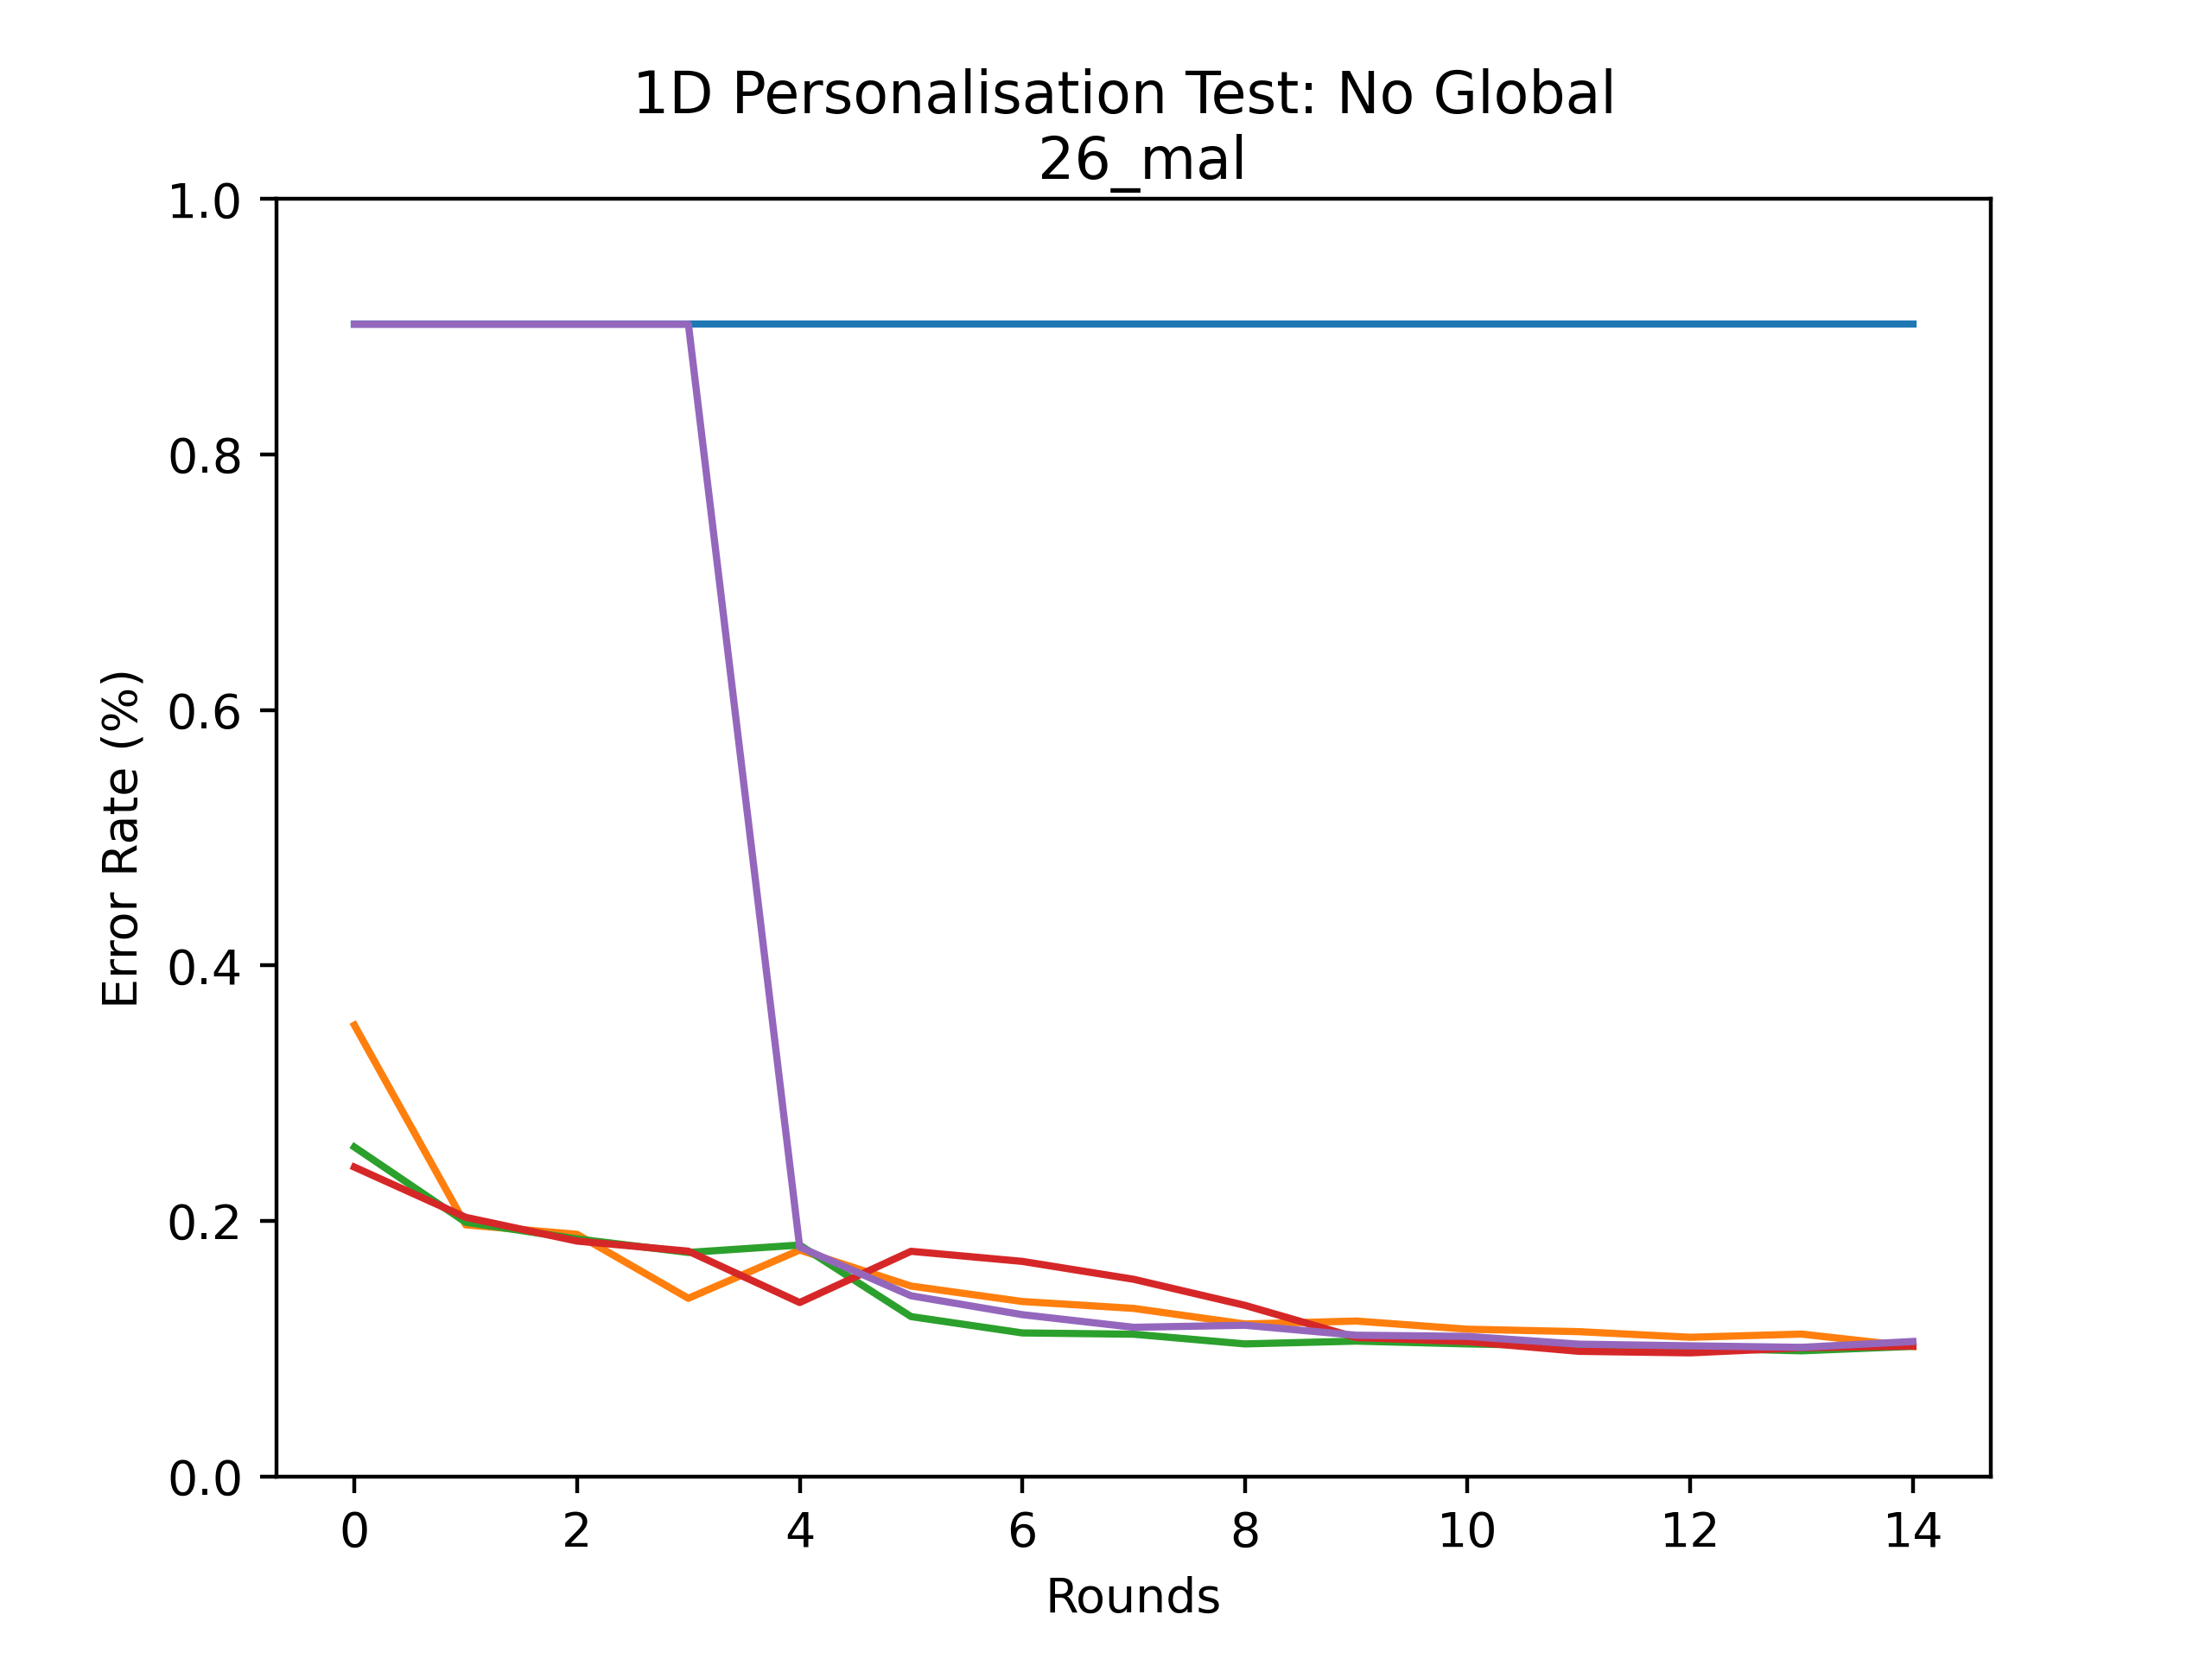
\includegraphics[scale=0.5]{my_agg/graphs/1d_no_global.png}
    \caption{1D PCA with the No Global Personalisation Method - 26 Malicious Clients}
	\label{fig:1D_no_global}
\end{figure}
The great thing about this is that this works at any level of malicious clients [\ref{fig:4D_no_global_1}] with the only noticeable difference being the random spikes that are caused because the labels assigned to clusters change.
It should be noted as well that the malicious clusters only ever contained malicious clients and the benign clusters only ever contained benign clients.
As such, there was no overlap or poisoning at all, not even by a single client.

\subsection{Free-Riders}
The final step in achieving all that was set out to do is to help conquer the free-riders.
The 2 options that are present are the no global method and the selective method.
\\ \\
For no global, the hope is that all of the free-riders will group together into their own cluster (due to their similarity) and will then not receive any contributions from proper clients.
Or at the very least, not get a properly converged model.
This might be harder due to the nature of the free-riders, and a few benign clients might be lost in the process if they get caught up in the same cluster as the free-riders.
\\ \\
For the selective method, it might be harder but the goal is to have the free-riders be in one of the 2 left-out clusters.
This allows for some leniency hopefully but at the same time there is more risk associated with that there is an increased chance of them stealing a good model if they are included in the selected group.
Either way, seeing how FedPADRC handles free-riders by itself as well as with malicious clients is what I shall test.
\\ \\
The no global method is the first testing point as if it can't work here, then it won't be able to handle the more lenient selective method.
I am also doing the testing with 4D PCA just to make sure that it isn't that causing any potential problems.
\\ \\
What ends up occurring is something quite magical and yet so obvious!
The free-riders get the same global model that is sent out at the very start of the process but they can't really make any realistic changes to it.
Therefore, every other client (whether or not it is malicious) will do some form of learning.
This then has a great distinctive effect of having the free-riders all look the same [\ref{fig:10mal10free_rep}] \textit{as well as} not being similar in any shape or form to the rest of the clients.
As such, it never even gets the opportunity to learn even a little bit, meaning that the free-riders fail in their goal [\ref{fig:no_15free}] as well as there being no intellectual property theft.
What's also good is that there wasn't even 1 free-rider that managed to sneak into the other clusters at any count of free-riders, they remained separate at all times.
\\ \\
It might end up being the case that FedPADRC isn't able to handle more than just one style of attack at any given time.
Alas, that is not the case!
Even when there is a combination of free-riders and malicious clients present [\ref{fig:no_13free_13mal}], it is not hindered in any-way-shape-or-form.
All that then happens is that there are 2 clusters that have awful performance with the 3 benign clusters making up all of the remaining benign clients.
\begin{figure}[htbp]
	\centering
    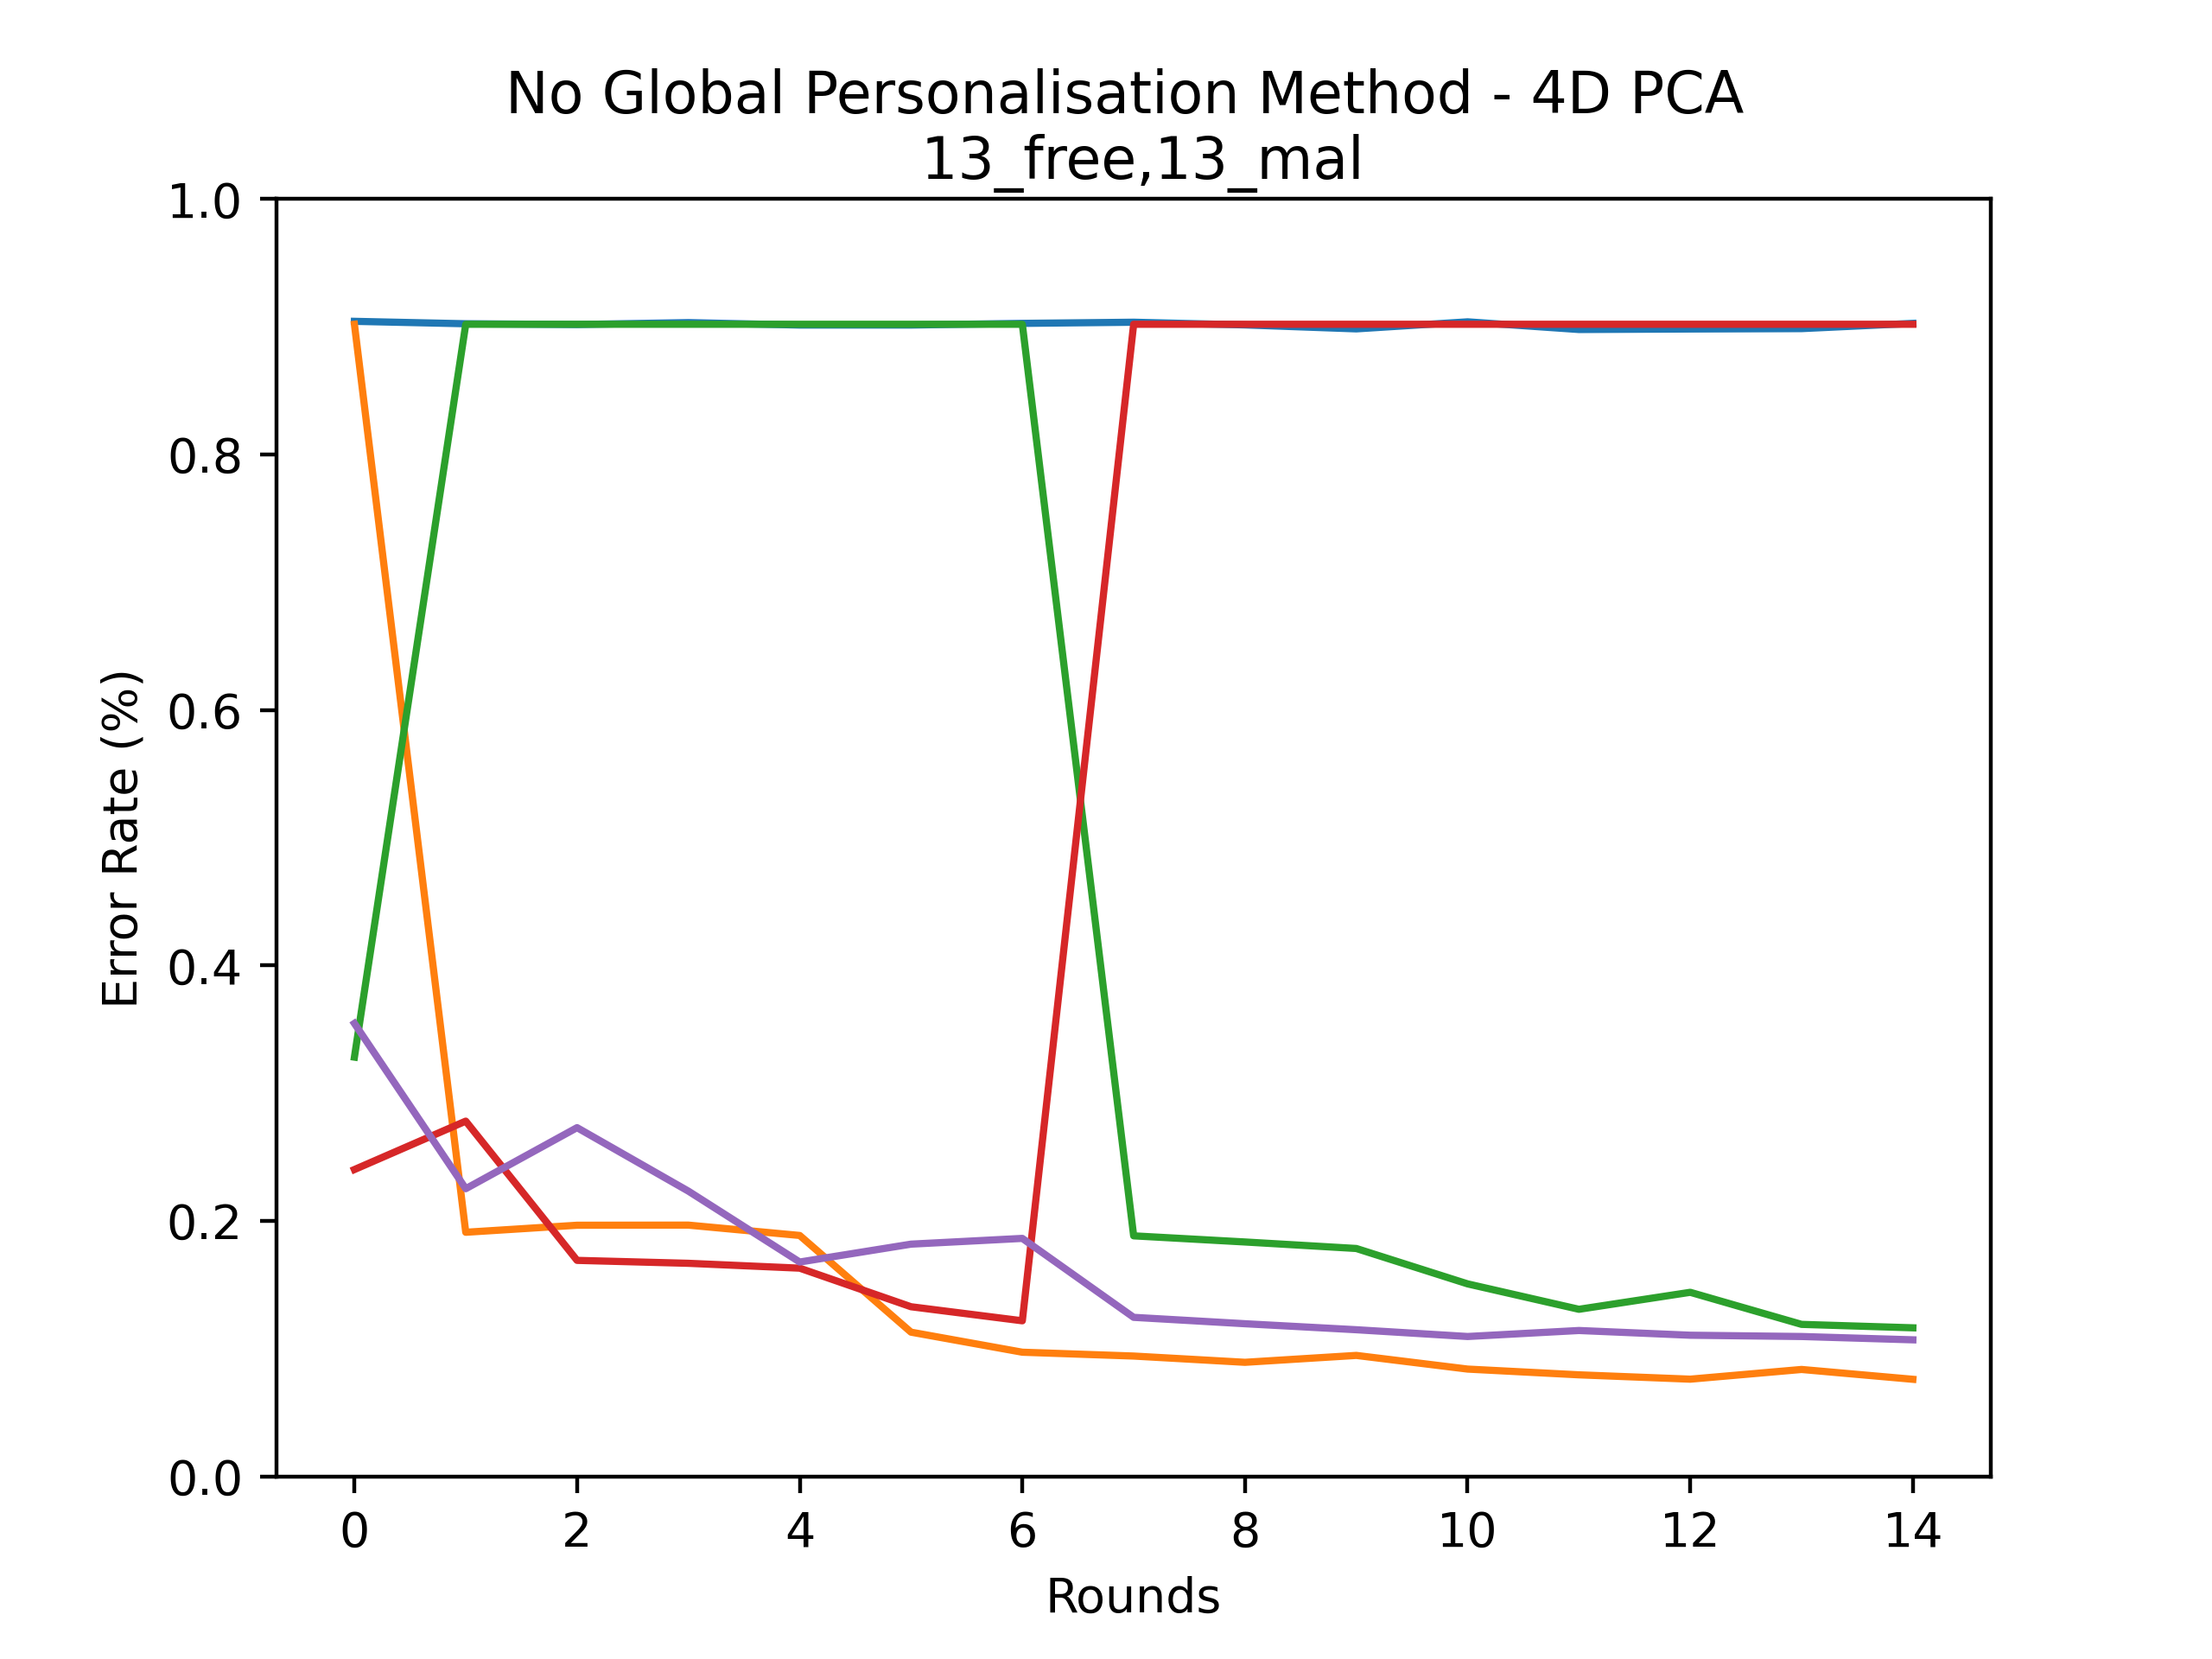
\includegraphics[scale=0.5]{my_agg/graphs/no_global_13free_13mal.png}
    \caption{4D PCA with the No Global Personalisation Method - 13 Free and 13 Malicious Clients. This shows that even under a combination attack, FedPADRC is able to hold its own.}
	\label{fig:no_13free_13mal}
\end{figure}
\\ \\
All of the above results are also emulated with the selective personalisation method.
This allows for the configurator of the federated system to be a bit more strict or lenient with the aggregation setup, allowing more variability for ensuring the robustness of the aggregation.

